% ============================================================
%  L03_mini5.tex  --  Payments and Fintech
%  5-Slide Teaser Arc: WHY > WHAT > HOW > WHERE > SO WHAT
%  Self-contained (no \input{} commands, no \includegraphics)
%  Compile: pdflatex L03_mini5.tex  (twice for overlays)
% ============================================================

\documentclass[aspectratio=169, 11pt]{beamer}
\usetheme{Madrid}
\usecolortheme{whale}
\usepackage{tikz,pgfplots,booktabs,multicol,amsmath}
\usetikzlibrary{arrows.meta,positioning,shapes.geometric,calc,decorations.pathmorphing}
\pgfplotsset{compat=1.18}

% ---- Colour palette ----------------------------------------
\definecolor{mlpurple}{HTML}{9467BD}
\definecolor{mlblue}{HTML}{1F77B4}
\definecolor{mlred}{HTML}{D62728}
\definecolor{mlorange}{HTML}{FF7F0E}
\definecolor{mlgreen}{HTML}{2CA02C}
\definecolor{mlgray}{HTML}{7F7F7F}
\definecolor{mlteal}{HTML}{0D7377}
\definecolor{mlcyan}{HTML}{14BDEB}

% ---- Beamer theme colours ----------------------------------
\setbeamercolor{structure}{fg=mlteal}
\setbeamercolor{palette primary}{bg=mlteal,fg=white}
\setbeamercolor{palette secondary}{bg=mlteal!80,fg=white}
\setbeamercolor{palette tertiary}{bg=mlteal!60,fg=white}
\setbeamercolor{frametitle}{bg=mlteal!10,fg=mlteal}
\setbeamercolor{title}{fg=white}
\setbeamercolor{subtitle}{fg=mlcyan!80}
\setbeamercolor{block title}{bg=mlteal,fg=white}
\setbeamercolor{block body}{bg=mlteal!8,fg=black}
\setbeamercolor{block title alerted}{bg=mlred!80,fg=white}
\setbeamercolor{block body alerted}{bg=mlred!8,fg=black}

% ---- Bottom-note command -----------------------------------
\newcommand{\bottomnote}[1]{%
  \vfill
  \begin{beamercolorbox}[wd=\textwidth,ht=2ex,dp=1ex]{palette primary}%
    \tiny\hspace{1em}#1%
  \end{beamercolorbox}}

% ---- Metadata ----------------------------------------------
\title{Payments and Fintech}
\subtitle{5-Slide Teaser}
\author{Joerg Osterrieder}
\institute{University of Zurich}
\date{Spring 2026}
\setbeamertemplate{navigation symbols}{}

% ============================================================
\begin{document}
% ============================================================

% -----------------------------------------------------------
%  TITLE FRAME (not counted in the 5)
% -----------------------------------------------------------
\begin{frame}
  \titlepage
  \bottomnote{Financial Technology (FinTech) -- MSc Course | University of Zurich | Spring 2026}
\end{frame}

% ===========================================================
%  SLIDE 1 of 5  --  WHY
%  Visual: TikZ comic -- evolution from barter to tap-to-pay
% ===========================================================
\begin{frame}{Why Payments? From Barter to Tap-to-Pay}

\begin{center}
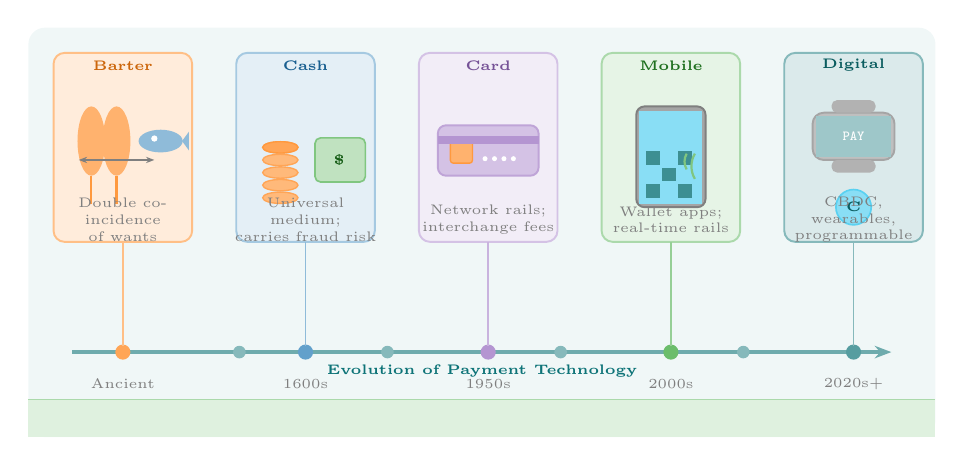
\begin{tikzpicture}[scale=0.80, every node/.style={font=\small}]

  % ---- Background strip ----
  \fill[mlteal!6, rounded corners=6pt] (-7.2,-2.9) rectangle (7.2,3.6);

  % ---- Ground line ----
  \fill[mlgreen!15] (-7.2,-2.9) rectangle (7.2,-2.3);
  \draw[mlgreen!40, line width=0.5pt] (-7.2,-2.3) -- (7.2,-2.3);

  % ---- Timeline arrow ----
  \draw[mlteal!60, -{Stealth[length=6pt]}, line width=1.4pt]
    (-6.5,-1.55) -- (6.5,-1.55);
  \node[font=\tiny\bfseries, text=mlteal] at (0,-1.85) {Evolution of Payment Technology};

  % ============ ERA 1: BARTER (far left) ============
  \fill[mlorange!15, rounded corners=4pt, draw=mlorange!50, line width=0.7pt]
    (-6.8,0.2) rectangle (-4.6,3.2);
  \node[font=\tiny\bfseries, text=mlorange!80!black] at (-5.7,3.0) {Barter};
  % Wheat sheaf (simple)
  \fill[mlorange!60] (-6.2,1.8) ellipse (0.22 and 0.55);
  \draw[mlorange!80, line width=0.8pt] (-6.2,1.25) -- (-6.2,0.8);
  \fill[mlorange!60] (-5.8,1.8) ellipse (0.22 and 0.55);
  \draw[mlorange!80, line width=0.8pt] (-5.8,1.25) -- (-5.8,0.8);
  % Arrow exchange
  \draw[mlgray, {Stealth[length=3pt]}-{Stealth[length=3pt]}, line width=0.8pt]
    (-6.4,1.5) -- (-5.2,1.5);
  % Fish
  \fill[mlblue!50] (-5.1,1.8) ellipse (0.35 and 0.18);
  \fill[mlblue!50] (-4.76,1.8) -- (-4.65,1.95) -- (-4.65,1.65) -- cycle;
  \fill[white] (-5.2,1.84) circle (0.05);
  % Problem label
  \node[font=\tiny, text=mlgray, align=center, text width=1.9cm]
    at (-5.7,0.55) {Double coincidence\\of wants};

  % ============ ERA 2: COINS/CASH (centre-left) ============
  \fill[mlblue!12, rounded corners=4pt, draw=mlblue!40, line width=0.7pt]
    (-3.9,0.2) rectangle (-1.7,3.2);
  \node[font=\tiny\bfseries, text=mlblue!80!black] at (-2.8,3.0) {Cash};
  % Coin stack
  \foreach \y in {0.9,1.1,1.3,1.5,1.7}{
    \fill[mlorange!55, draw=mlorange!70, line width=0.5pt]
      (-3.2,\y) ellipse (0.28 and 0.09);
  }
  \fill[mlorange!70, draw=mlorange!80, line width=0.5pt]
    (-3.2,1.7) ellipse (0.28 and 0.09);
  % Banknote
  \fill[mlgreen!30, draw=mlgreen!60, line width=0.6pt, rounded corners=2pt]
    (-2.65,1.15) rectangle (-1.85,1.85);
  \node[font=\tiny\bfseries, text=mlgreen!60!black] at (-2.25,1.50) {\$};
  % Label
  \node[font=\tiny, text=mlgray, align=center, text width=1.9cm]
    at (-2.8,0.55) {Universal medium;\\carries fraud risk};

  % ============ ERA 3: CARD (centre) ============
  \fill[mlpurple!12, rounded corners=4pt, draw=mlpurple!40, line width=0.7pt]
    (-1.0,0.2) rectangle (1.2,3.2);
  \node[font=\tiny\bfseries, text=mlpurple!80!black] at (0.1,3.0) {Card};
  % Credit card shape
  \fill[mlpurple!40, draw=mlpurple!60, line width=0.7pt, rounded corners=3pt]
    (-0.7,1.25) rectangle (0.9,2.05);
  % Chip
  \fill[mlorange!60, draw=mlorange!80, line width=0.5pt, rounded corners=1pt]
    (-0.5,1.45) rectangle (-0.15,1.85);
  % Stripe
  \fill[mlpurple!70] (-0.7,1.75) rectangle (0.9,1.88);
  % Card number dots
  \foreach \x in {0.05,0.2,0.35,0.5}{
    \fill[white] (\x,1.52) circle (0.04);
  }
  % Label
  \node[font=\tiny, text=mlgray, align=center, text width=1.9cm]
    at (0.1,0.55) {Network rails;\\interchange fees};

  % ============ ERA 4: MOBILE (centre-right) ============
  \fill[mlgreen!12, rounded corners=4pt, draw=mlgreen!40, line width=0.7pt]
    (1.9,0.2) rectangle (4.1,3.2);
  \node[font=\tiny\bfseries, text=mlgreen!70!black] at (3.0,3.0) {Mobile};
  % Phone body
  \fill[mlgray!70, draw=mlgray, line width=0.7pt, rounded corners=3pt]
    (2.45,0.75) rectangle (3.55,2.35);
  \fill[mlcyan!50] (2.50,0.80) rectangle (3.50,2.28);
  % QR code on screen (simplified grid)
  \foreach \r in {0,1,2}{\foreach \c in {0,1,2}{
    \pgfmathparse{mod(\r+\c,2)==0 ? 1 : 0}
    \ifnum\pgfmathresult=1
      \fill[mlteal!80]
        ({2.60+\c*0.26},{0.90+\r*0.26}) rectangle
        ({2.82+\c*0.26},{1.12+\r*0.26});
    \fi
  }}
  % NFC symbol
  \draw[mlgreen!60, line width=0.8pt] (3.25,1.6) arc(150:210:0.25);
  \draw[mlgreen!60, line width=0.8pt] (3.38,1.6) arc(150:210:0.40);
  % Label
  \node[font=\tiny, text=mlgray, align=center, text width=1.9cm]
    at (3.0,0.55) {Wallet apps;\\real-time rails};

  % ============ ERA 5: TAP-TO-PAY / CBDC (far right) ============
  \fill[mlteal!15, rounded corners=4pt, draw=mlteal!50, line width=0.7pt]
    (4.8,0.2) rectangle (7.0,3.2);
  \node[font=\tiny\bfseries, text=mlteal!80!black] at (5.9,3.0) {Digital};
  % Wearable / watch
  \fill[mlgray!50, draw=mlgray!70, line width=0.7pt, rounded corners=4pt]
    (5.25,1.5) rectangle (6.55,2.25);
  \fill[mlteal!40] (5.30,1.55) rectangle (6.50,2.20);
  \node[font=\tiny\bfseries, text=white] at (5.9,1.875) {\texttt{PAY}};
  % Strap top/bottom
  \fill[mlgray!60, rounded corners=2pt] (5.55,2.25) rectangle (6.25,2.45);
  \fill[mlgray!60, rounded corners=2pt] (5.55,1.30) rectangle (6.25,1.50);
  % CBDC coin
  \fill[mlcyan!50, draw=mlcyan!70, line width=0.6pt] (5.9,0.75) circle (0.28);
  \node[font=\tiny\bfseries, text=mlteal!80!black] at (5.9,0.75) {C};
  % Label
  \node[font=\tiny, text=mlgray, align=center, text width=1.9cm]
    at (5.9,0.55) {CBDC, wearables,\\programmable};

  % ---- Connecting arrows on timeline ----
  \foreach \x in {-3.85,-1.5,1.25,4.15}{
    \fill[mlteal!50] (\x,-1.55) circle (0.10);
  }
  \fill[mlorange!70] (-5.7,-1.55) circle (0.12);
  \fill[mlblue!70]   (-2.8,-1.55) circle (0.12);
  \fill[mlpurple!70] ( 0.1,-1.55) circle (0.12);
  \fill[mlgreen!70]  ( 3.0,-1.55) circle (0.12);
  \fill[mlteal!70]   ( 5.9,-1.55) circle (0.12);

  % Tick lines from circles to boxes
  \draw[mlorange!50, line width=0.6pt] (-5.7,-1.45) -- (-5.7,0.2);
  \draw[mlblue!50,   line width=0.6pt] (-2.8,-1.45) -- (-2.8,0.2);
  \draw[mlpurple!50, line width=0.6pt] ( 0.1,-1.45) -- ( 0.1,0.2);
  \draw[mlgreen!50,  line width=0.6pt] ( 3.0,-1.45) -- ( 3.0,0.2);
  \draw[mlteal!50,   line width=0.6pt] ( 5.9,-1.45) -- ( 5.9,0.2);

  % Year labels
  \node[font=\tiny, text=mlgray] at (-5.7,-2.05) {Ancient};
  \node[font=\tiny, text=mlgray] at (-2.8,-2.05) {1600s};
  \node[font=\tiny, text=mlgray] at ( 0.1,-2.05) {1950s};
  \node[font=\tiny, text=mlgray] at ( 3.0,-2.05) {2000s};
  \node[font=\tiny, text=mlgray] at ( 5.9,-2.05) {2020s+};

\end{tikzpicture}
\end{center}

\bottomnote{Slide 1/5 --- WHY | Every payment era solved the friction of the prior one -- fintech targets the remaining frictions of speed, cost, and access.}
\end{frame}

% ===========================================================
%  SLIDE 2 of 5  --  WHAT
%  Visual: booktabs table -- payment methods comparison
% ===========================================================
\begin{frame}[shrink=5]{What Are the Payment Methods? A Comparative View}

\vspace{-0.1em}
\begin{center}
\textcolor{mlteal}{\textbf{\small Illustrative Comparison of Payment Methods Across Key Dimensions}}
\vspace{0.5em}

\scriptsize
\setlength{\tabcolsep}{5pt}
\renewcommand{\arraystretch}{1.30}
\begin{tabular}{@{}lp{2.1cm}p{2.0cm}p{2.0cm}p{2.0cm}p{2.0cm}@{}}
  \toprule
  \textbf{Method} & \textbf{Settlement Speed} & \textbf{Cost to Merchant} & \textbf{Privacy} & \textbf{Global Reach} & \textbf{Offline?} \\
  \midrule
  \textbf{Cash} &
    Instant (T+0) &
    Near zero &
    \textcolor{mlgreen!70!black}{High} (anonymous) &
    Domestic only &
    \textcolor{mlgreen!70!black}{Yes} \\[2pt]

  \textbf{Debit / Credit Card} &
    T+1 to T+2 &
    1--3\% interchange &
    \textcolor{mlorange!80!black}{Low} (tracked) &
    International &
    \textcolor{mlred}{No} \\[2pt]

  \textbf{Mobile Wallet} &
    Near-instant &
    0.5--1.5\% &
    \textcolor{mlorange!80!black}{Low} (data collected) &
    Growing &
    \textcolor{mlorange!80!black}{Partial} \\[2pt]

  \textbf{Bank Transfer / RTGS} &
    Instant or T+1 &
    Low (flat fee) &
    \textcolor{mlorange!80!black}{Moderate} &
    Limited by rails &
    \textcolor{mlred}{No} \\[2pt]

  \textbf{Stablecoin} &
    Minutes (T+0) &
    Very low &
    \textcolor{mlorange!80!black}{Pseudonymous} &
    Global &
    \textcolor{mlred}{No} \\[2pt]

  \textbf{CBDC} &
    Instant (T+0) &
    Potentially zero &
    \textcolor{mlred}{Low} (state visibility) &
    Bilateral CBs &
    \textcolor{mlgreen!70!black}{Designed for it} \\
  \bottomrule
\end{tabular}
\end{center}

\vspace{0.3em}
\begin{columns}[T]
\begin{column}{0.48\textwidth}
  \begin{block}{No Single Winner}
    \scriptsize
    Each method trades off cost, speed, privacy, and reach differently.
    The ``best'' payment method depends on the \textbf{use case}:
    micro-payment, cross-border, retail, or wholesale.
  \end{block}
\end{column}
\begin{column}{0.48\textwidth}
  \begin{alertblock}{\scriptsize The Friction Lens}
    \scriptsize
    Fintech competes by \textbf{reducing one friction at a time}:
    cards cut cash-handling cost; wallets cut card friction;
    stablecoins cut FX conversion delays.
  \end{alertblock}
\end{column}
\end{columns}

\bottomnote{Slide 2/5 --- WHAT | Payments = information + value transfer. Reducing friction on either dimension is where fintech creates value.}
\end{frame}

% ===========================================================
%  SLIDE 3 of 5  --  HOW
%  Visual: TikZ diagram -- simplified four-party payment model
% ===========================================================
\begin{frame}{How Do Card Payments Flow? The Four-Party Model}

\begin{center}
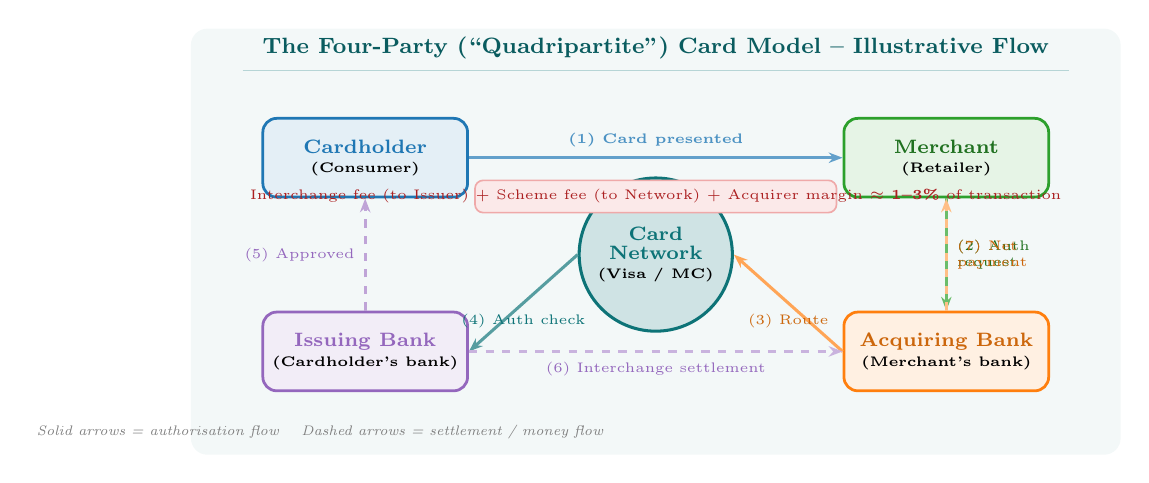
\begin{tikzpicture}[
    scale=0.82,
    box/.style={rectangle, rounded corners=5pt, minimum width=2.6cm,
                minimum height=1.0cm, align=center, font=\scriptsize\bfseries,
                line width=1.0pt, draw},
    arr/.style={-{Stealth[length=5pt]}, line width=1.1pt},
    revarr/.style={{Stealth[length=5pt]}-, line width=1.1pt},
    every node/.style={font=\small}
  ]

  % ---- Background ----
  \fill[mlteal!5, rounded corners=6pt] (-7.2,-3.2) rectangle (7.2,3.4);

  % ---- Title ----
  \node[font=\footnotesize\bfseries, text=mlteal!80!black] at (0,3.1)
    {The Four-Party (``Quadripartite'') Card Model -- Illustrative Flow};
  \draw[mlteal!30, line width=0.4pt] (-6.4,2.75) -- (6.4,2.75);

  % ============ FOUR NODES ============

  % Cardholder (top-left)
  \node[box, fill=mlblue!12, draw=mlblue]
    (CH) at (-4.5,1.4) {\textcolor{mlblue}{Cardholder}\\[-1pt]\tiny(Consumer)};

  % Merchant (top-right)
  \node[box, fill=mlgreen!12, draw=mlgreen]
    (ME) at (4.5,1.4) {\textcolor{mlgreen!70!black}{Merchant}\\[-1pt]\tiny(Retailer)};

  % Issuing Bank (bottom-left)
  \node[box, fill=mlpurple!12, draw=mlpurple]
    (IB) at (-4.5,-1.6) {\textcolor{mlpurple}{Issuing Bank}\\[-1pt]\tiny(Cardholder's bank)};

  % Acquiring Bank (bottom-right)
  \node[box, fill=mlorange!12, draw=mlorange]
    (AB) at (4.5,-1.6) {\textcolor{mlorange!80!black}{Acquiring Bank}\\[-1pt]\tiny(Merchant's bank)};

  % Card Network (centre)
  \node[circle, fill=mlteal!20, draw=mlteal, line width=1.1pt,
        minimum size=1.6cm, align=center, font=\scriptsize\bfseries]
    (CN) at (0,-0.1) {\textcolor{mlteal}{Card}\\[-1pt]\textcolor{mlteal}{Network}\\[-1pt]\tiny(Visa / MC)};

  % ============ ARROWS ============

  % 1. Cardholder pays Merchant (top horizontal)
  \draw[arr, mlblue!70] (CH.east) -- (ME.west)
    node[midway, above, font=\tiny\bfseries, text=mlblue!80] {(1) Card presented};

  % 2. Merchant --> Acquiring Bank (right vertical, auth request down)
  \draw[arr, mlgreen!70] (ME.south) -- (AB.north)
    node[midway, right, font=\tiny, text=mlgreen!70!black, align=left]
    {(2) Auth\\request};

  % 3. Acquiring Bank --> Card Network
  \draw[arr, mlorange!70] (AB.west) -- (CN.east)
    node[midway, below, font=\tiny, text=mlorange!80!black] {(3) Route};

  % 4. Card Network --> Issuing Bank
  \draw[arr, mlteal!70] (CN.west) -- (IB.east)
    node[midway, below, font=\tiny, text=mlteal] {(4) Auth check};

  % 5. Issuing Bank approves back through network (dashed)
  \draw[arr, mlpurple!60, dashed] (IB.north) -- (CH.south)
    node[midway, left, font=\tiny, text=mlpurple] {(5) Approved};

  % 6. Settlement: Issuing --> Acquiring (bottom horizontal, dashed)
  \draw[arr, mlpurple!50, dashed] (IB.east) -- (AB.west)
    node[midway, below, font=\tiny, text=mlpurple] {(6) Interchange settlement};

  % 7. Acquiring --> Merchant net of fees (dashed)
  \draw[arr, mlorange!50, dashed] (AB.north) -- (ME.south)
    node[midway, right, font=\tiny, text=mlorange!80!black, align=left]
    {(7) Net\\payment};

  % ============ FEE ANNOTATIONS ============
  \fill[mlred!10, rounded corners=3pt, draw=mlred!40, line width=0.6pt]
    (-2.8,0.55) rectangle (2.8,1.05);
  \node[font=\tiny, text=mlred!80!black, align=center]
    at (0,0.80)
    {Interchange fee (to Issuer) + Scheme fee (to Network) + Acquirer margin
     $\approx$ \textbf{1--3\%} of transaction};

  % ============ LEGEND ============
  \node[font=\tiny\itshape, text=mlgray, align=left]
    at (-5.2,-2.85) {Solid arrows = authorisation flow \quad Dashed arrows = settlement / money flow};

\end{tikzpicture}
\end{center}

\bottomnote{Slide 3/5 --- HOW | The four-party model dates to the 1960s. Fintech attacks each leg: neo-banks on issuing, PayFacs on acquiring, stablecoins on the network.}
\end{frame}

% ===========================================================
%  SLIDE 4 of 5  --  WHERE
%  Visual: pgfplots bar chart -- illustrative merchant costs
% ===========================================================
\begin{frame}{Where Does the Money Go? Illustrative Merchant Cost by Payment Type}

\vspace{-0.4em}
\begin{center}
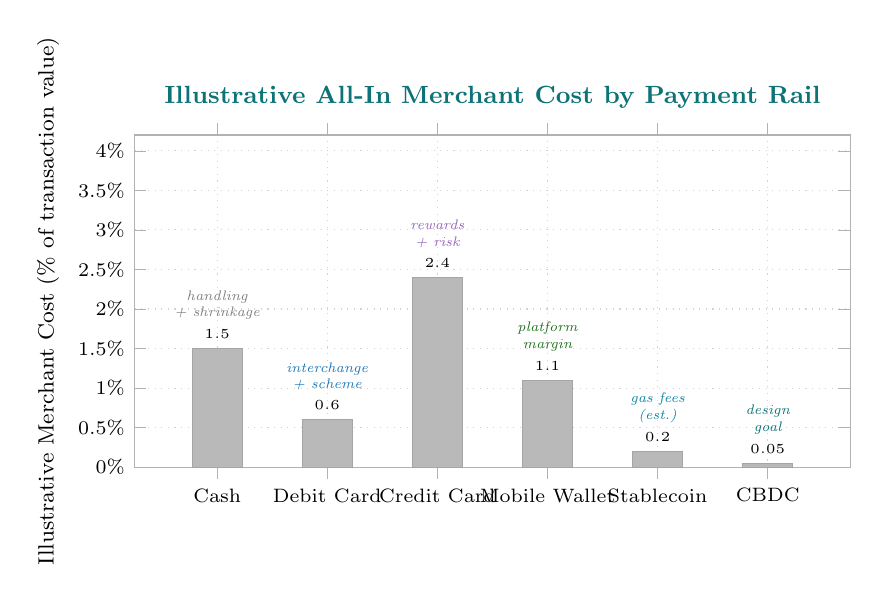
\begin{tikzpicture}
\begin{axis}[
    ybar,
    bar width=18pt,
    width=0.88\textwidth,
    height=5.8cm,
    enlarge x limits=0.15,
    ylabel={\footnotesize Illustrative Merchant Cost (\% of transaction value)},
    ylabel style={font=\scriptsize},
    ymin=0, ymax=4.2,
    ytick={0,0.5,1.0,1.5,2.0,2.5,3.0,3.5,4.0},
    yticklabel style={font=\scriptsize},
    yticklabel={\pgfmathprintnumber[fixed,precision=1]{\tick}\%},
    symbolic x coords={Cash, Debit Card, Credit Card, Mobile Wallet, Stablecoin, CBDC},
    xtick=data,
    xticklabel style={font=\scriptsize, align=center, text width=1.8cm},
    grid=major,
    grid style={dotted, mlgray!35},
    axis line style={mlgray!60},
    tick style={mlgray!60},
    title={\small Illustrative All-In Merchant Cost by Payment Rail},
    title style={font=\small\bfseries, color=mlteal},
    nodes near coords,
    nodes near coords style={font=\tiny\bfseries, color=black},
    every node near coord/.append style={/pgf/number format/fixed, /pgf/number format/precision=2}
  ]

  % Cash: handling, cash-in-transit, shrinkage ~1.5%
  \addplot[fill=mlgray!55, draw=mlgray!70] coordinates {
    (Cash,          1.50)
    (Debit Card,    0.60)
    (Credit Card,   2.40)
    (Mobile Wallet, 1.10)
    (Stablecoin,    0.20)
    (CBDC,          0.05)
  };

  % Cost component labels
  \node[font=\tiny\itshape, text=mlgray, align=center]
    at (axis cs:Cash, 2.05)
    {handling\\+ shrinkage};
  \node[font=\tiny\itshape, text=mlblue, align=center]
    at (axis cs:Debit Card, 1.15)
    {interchange\\+ scheme};
  \node[font=\tiny\itshape, text=mlpurple, align=center]
    at (axis cs:Credit Card, 2.95)
    {rewards\\+ risk};
  \node[font=\tiny\itshape, text=mlgreen!70!black, align=center]
    at (axis cs:Mobile Wallet, 1.65)
    {platform\\margin};
  \node[font=\tiny\itshape, text=mlcyan!70!black, align=center]
    at (axis cs:Stablecoin, 0.75)
    {gas fees\\(est.)};
  \node[font=\tiny\itshape, text=mlteal, align=center]
    at (axis cs:CBDC, 0.60)
    {design\\goal};

\end{axis}
\end{tikzpicture}
\end{center}

\vspace{-0.5em}
{\tiny\textcolor{mlgray}{\textit{All figures are purely illustrative for teaching purposes. Actual costs vary by country, volume, contract, and product type.}}}

\bottomnote{Slide 4/5 --- WHERE | Merchant cost is the competitive battleground: every basis point saved at scale is a significant margin improvement for fintech rails.}
\end{frame}

% ===========================================================
%  SLIDE 5 of 5  --  SO WHAT
%  Visual: Payment evaluation framework -- 5 key questions
% ===========================================================
\begin{frame}{So What? A Framework for Evaluating Any Payment System}

\begin{center}
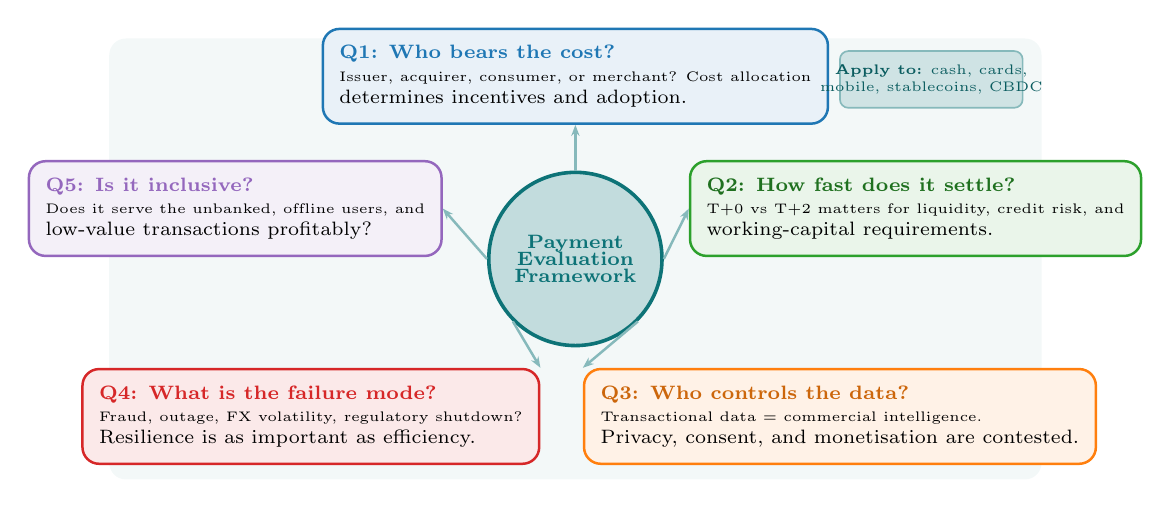
\begin{tikzpicture}[
    scale=0.80,
    qbox/.style={rectangle, rounded corners=6pt, minimum width=5.2cm,
                 minimum height=1.05cm, align=left, font=\scriptsize,
                 line width=0.9pt, draw, inner sep=6pt},
    every node/.style={font=\small}
  ]

  % ---- Background ----
  \fill[mlteal!5, rounded corners=6pt] (-7.4,-3.5) rectangle (7.4,3.5);

  % ---- Central hub ----
  \node[circle, fill=mlteal!25, draw=mlteal, line width=1.3pt,
        minimum size=2.2cm, align=center, font=\scriptsize\bfseries]
    (HUB) at (0,0)
    {\textcolor{mlteal}{Payment}\\[-2pt]\textcolor{mlteal}{Evaluation}\\[-2pt]\textcolor{mlteal}{Framework}};

  % ============ 5 QUESTION BOXES (arranged radially) ============

  % Q1: TOP  -- Who pays the cost?
  \node[qbox, fill=mlblue!10, draw=mlblue]
    (Q1) at (0, 2.9)
    {\textcolor{mlblue}{\bfseries Q1: Who bears the cost?}\\
     \tiny Issuer, acquirer, consumer, or merchant? Cost allocation\\determines incentives and adoption.};

  % Q2: RIGHT -- How fast does it settle?
  \node[qbox, fill=mlgreen!10, draw=mlgreen]
    (Q2) at (5.4, 0.8)
    {\textcolor{mlgreen!70!black}{\bfseries Q2: How fast does it settle?}\\
     \tiny T+0 vs T+2 matters for liquidity, credit risk, and\\working-capital requirements.};

  % Q3: BOTTOM-RIGHT -- Who controls the data?
  \node[qbox, fill=mlorange!10, draw=mlorange]
    (Q3) at (4.2,-2.5)
    {\textcolor{mlorange!80!black}{\bfseries Q3: Who controls the data?}\\
     \tiny Transactional data = commercial intelligence.\\Privacy, consent, and monetisation are contested.};

  % Q4: BOTTOM-LEFT -- What is the failure mode?
  \node[qbox, fill=mlred!10, draw=mlred]
    (Q4) at (-4.2,-2.5)
    {\textcolor{mlred}{\bfseries Q4: What is the failure mode?}\\
     \tiny Fraud, outage, FX volatility, regulatory shutdown?\\Resilience is as important as efficiency.};

  % Q5: LEFT -- Is it inclusive?
  \node[qbox, fill=mlpurple!10, draw=mlpurple]
    (Q5) at (-5.4, 0.8)
    {\textcolor{mlpurple}{\bfseries Q5: Is it inclusive?}\\
     \tiny Does it serve the unbanked, offline users, and\\low-value transactions profitably?};

  % ---- Spoke arrows from hub ----
  \draw[mlteal!50, -{Stealth[length=4pt]}, line width=0.9pt]
    (HUB.north)      -- (Q1.south);
  \draw[mlteal!50, -{Stealth[length=4pt]}, line width=0.9pt]
    (HUB.east)       -- (Q2.west);
  \draw[mlteal!50, -{Stealth[length=4pt]}, line width=0.9pt]
    (HUB.south east) -- (Q3.north west);
  \draw[mlteal!50, -{Stealth[length=4pt]}, line width=0.9pt]
    (HUB.south west) -- (Q4.north east);
  \draw[mlteal!50, -{Stealth[length=4pt]}, line width=0.9pt]
    (HUB.west)       -- (Q5.east);

  % ---- Corner tag ----
  \fill[mlteal!20, rounded corners=3pt, draw=mlteal!50, line width=0.6pt]
    (4.2,2.4) rectangle (7.1,3.3);
  \node[font=\tiny, text=mlteal!80!black, align=center]
    at (5.65,2.85)
    {\textbf{Apply to:} cash, cards,\\mobile, stablecoins, CBDC};

\end{tikzpicture}
\end{center}

\bottomnote{Slide 5/5 --- SO WHAT | Five questions, any rail: cost allocation, settlement speed, data control, failure modes, and inclusion -- evaluate any payment system with this lens.}
\end{frame}

% ===========================================================
%  END
% ===========================================================
\end{document}
